
%dash pattern=on 5pt off 2pt
%[fill = white, rounded corners = 5pt, inner sep=0.8pt]
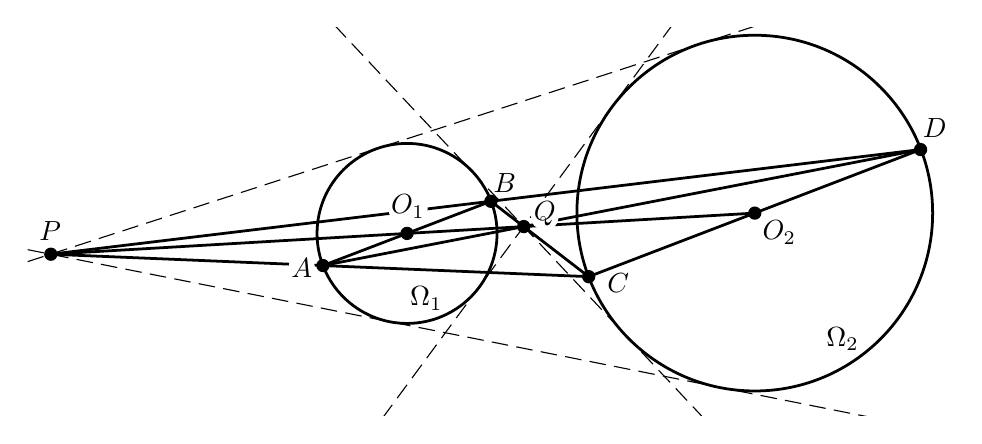
\begin{tikzpicture}[scale = 0.3]
    \clip(-18.5,-3.66) rectangle (20.71,12.77);
    \draw [line width=1pt] (-2.44,4.06) circle (3.81cm);
    \draw [line width=1pt] (12.28,4.92) circle (7.53cm);
    \draw [dash pattern=on 6pt off 3pt, domain=-18.5:20.71] plot(\x,{(-15.21--2.31*\x)/-2.17});
    \draw [dash pattern=on 6pt off 3pt, domain=-18.5:20.71] plot(\x,{(-1.81-2.55*\x)/-1.88});
    \draw [dash pattern=on 6pt off 3pt, domain=-18.5:20.71] plot(\x,{(-4.4-2.85*\x)/14.33});
    \draw [dash pattern=on 6pt off 3pt, domain=-18.5:20.71] plot(\x,{(--123.1--4.5*\x)/13.9});
    \draw [line width=1pt] (-17.52,3.18)-- (5.25,2.23);
    \draw [line width=1pt] (-17.52,3.18)-- (19.3,7.61);
    \draw [line width=1pt] (-17.52,3.18)-- (12.28,4.92);
    \draw [line width=1pt] (-6,2.7)-- (1.11,5.42);
    \draw [line width=1pt] (5.25,2.23)-- (19.3,7.61);
    \draw [line width=1pt] (-6,2.7)-- (19.3,7.61);
    \draw [line width=1pt] (5.25,2.23)-- (1.11,5.42);
    \begin{scriptsize}
        \normalsize
        \fill [color=black] (-2.44,4.06) circle (8pt);
        \draw[color=black] (-2.4,5.2) node[fill = white, rounded corners = 4pt, inner sep = 1pt] {$O_1$};
        \fill [color=black] (-6,2.7) circle (8pt);
        \draw[color=black] (-6.9,2.6) node[fill = white, rounded corners = 4pt, inner sep = 1pt] {$A$};
        \fill [color=black] (1.11,5.42) circle (8pt);
        \draw[color=black] (1.7,6.2) node[fill = white, rounded corners = 4pt, inner sep = 1pt] {$B$};
        \fill [color=black] (5.25,2.23) circle (8pt);
        \draw[color=black] (6.5,1.95) node[fill = white, rounded corners = 4pt, inner sep = 1pt] {$C$};
        \fill [color=black] (12.28,4.92) circle (8pt);
        \draw[color=black] (13.32,4.1) node[fill = white, rounded corners = 4pt, inner sep = 1pt] {$O_2$};
        \fill [color=black] (19.3,7.61) circle (8pt);
        \draw[color=black] (19.9,8.5) node[fill = white, rounded corners = 4pt, inner sep = 1pt] {$D$};
        \fill [color=black] (2.5,4.35) circle (8pt);
        \draw[color=black] (3.39,4.88) node[fill = white, rounded corners = 4pt, inner sep = 1pt] {$Q$};
        \fill [color=black] (-17.52,3.18) circle (8pt);
        \draw[color=black] (-17.55,4.14) node[fill = white, rounded corners = 4pt, inner sep = 1pt] {$P$};

        \draw[color=black] (-1.62,1.3) node[fill = white, rounded corners = 4pt, inner sep = 1pt] {$\Omega_1$};
        \draw[color=black] (16, -0.4) node[fill = white, rounded corners = 4pt, inner sep = 1pt] {$\Omega_2$};
    \end{scriptsize}
\end{tikzpicture}